% Change project title and subtitle here
% Also dont forget to update project team members in title.tex
\def\paperTitle{Integrated Project \#3}
\def\paperSubTitle{Angular Oscillations of the Rigid Body}

% Document configuration
% Do not change anything here unless you know what you are doing
% Go to line 53 to start adding your content
\documentclass[
	12pt,twoside,a4paper
]{report}

% Some useful packages to get you started
% You can add more packages here if you need them
\usepackage{graphicx}
\usepackage[margin=1in]{geometry}
\usepackage{fancyhdr}
\usepackage[utf8]{inputenc}
\usepackage{etoc}
\usepackage{xcolor, soul}
\usepackage{listings}
\usepackage{amsmath}
\usepackage{lipsum}
\usepackage{hyperref}
\usepackage[style=apa, backend=biber]{biblatex}

\addbibresource{references.bib}
\DeclareLanguageMapping{english}{english-apa}

\sethlcolor{yellow}

\fancypagestyle{plain}{
	\fancyhf{}
	\fancyhead[l]{IP\#3}
	\fancyhead[c]{Angular Oscillations}
	\fancyhead[r]{January 18, 2024}
	\fancyfoot[le, ro]{Page \thepage}
	\fancyfoot[c]{January 18, 2024}
	\setlength{\headheight}{15pt}
	\renewcommand{\headrulewidth}{0.2pt}
	\renewcommand{\footrulewidth}{0.2pt}
}	

\thispagestyle{plain}

\renewcommand{\etocaftertitlehook}{\thispagestyle{plain}}
\renewcommand{\etocaftertochook}{\thispagestyle{plain}}

\begin{document}
	% Title page
% Do not change anything here unless you know what you are doing
% Go to line 29 to change project team members
\begin{center}
	
\includegraphics[width=0.4\textwidth]{assets/agu.png}

	\Huge
	\textbf{\paperTitle}

	\vspace{0.3cm}
	\Huge
	\paperSubTitle{}

	\vspace{0.8cm}
	\large
	\vspace{0.5cm}
	\LARGE
	\vspace{1.5cm}
	\textbf{}
	\vfill
	\vspace{0.8cm}
	\Large
\end{center}

\begin{tabbing}
	\hspace*{1em}\= \hspace*{8em} \= \kill
	\> Barış DEMİRCİ \> agu@338.rocks \\
	\> \> \\
	\> January 18, 2024 \> \\
\end{tabbing}


	\tableofcontents

	% Start adding your content here
	% These are just some examples to start with
	\chapter{Abstract}

This report investigates the torsional oscillations of a cylinder cup suspended on an elastic string. We determined the moment of inertia, torsion modulus, and checked the conservation of energy based on experimental measurements.

	\chapter{Introduction}

\section{Objective}

The primary objective of this experiment is to explore the torsional oscillations of a cylindrical cup suspended on an elastic wire. The specific goals include the determination of the moment of inertia ($I$) of the cylindrical cup using the disk method, the calculation of the torsion modulus ($J$) of the string, and the experimental verification of the conservation of energy.

\section{Context}

Torsional oscillations are a result of a body suspended on an elastic wire undergoing oscillations due to the moment of elastic forces. The relationship between the period ($T$), moment of inertia ($I$), and torsion modulus ($J$) is expressed by this equation: 

\[ T = 2\pi \sqrt{\frac{I}{J}}\]

\noindent According to the conservation law, the kinetic energy of the rotational motion of the pendulum is should be converted into potential energy:

\[ \frac{1}{2}I\omega^2 = \frac{1}{2}J\phi_{\max}^2\]

	\chapter{Experimental Setup}

\section{Materials}

\begin{itemize}
    \item{\textbf{Utensil:}} A cylindrical cup with the following dimensions:
    \begin{itemize}
        \item \textbf{Mass} ($m$): $118g$
        \item \textbf{Inner Radius} ($r_1$): $18cm$
        \item \textbf{Outer Radius} ($r_2$): $20cm$
        \item \textbf{Height} ($h$): $9cm$
    \end{itemize}
    \item{\textbf{Suspension:}} An elastic string attached to the top of the cup.
\end{itemize}

\section{Procedure}

\begin{itemize}
    \item{\textbf{Setup:}} Assemble the angular pendulum setup with the cylindrical cup attached to an elastic lightweight suspension.
    \item{\textbf{Measurements:}} Record the relevant dimensions of the cylindrical cup, including the inner and outer radii.
    \item{\textbf{Angular Displacement:}} Release the cylindrical cup to measure angular displacement ($\phi_{\max}$) and record the corresponding angular velocity ($\omega$).
    \item{\textbf{Data Collection:}} Document all experimental data for subsequent analysis.
\end{itemize}

\newpage
\thispagestyle{plain}

\section{Data}

The data below is obtained from the experimental setup described above. The data is used to calculate the moment of inertia ($I$) of the cylindrical cup and torsion modulus ($J$) of the string. Here is the experiment video: \url{https://youtu.be/hGKMeG9jghA}

\bigbreak{}
\bigbreak{}

\begin{center}
    \begin{tabular}{ |l||l|  }
        \hline
    
        Data & Value \\
    
        \hline
    
        Mass ($m$) & $118~g$ \\
        Frequency ($f$) & $\frac{1}{3}~Hz$ \\
        Maximum angle of twist ($\phi_{\max}$) & $360^\circ$ \\
        Angular velocity after impact ($\omega$) & $19~rad/s$ \\
        \hline
    \end{tabular}    
\end{center}


	\chapter{Mathematical Analysis}

\section{Moment of Inertia Calculation}

The method of moment of inertia ($I$) calculation that we chosed is the disk method. This method involves summing up the contributions of many small disk elements, each with its own moment of inertia. 

\bigbreak{}

For a cylindrical cup, the most appropriate integration method to calculate the moment of inertia is the disk method. The disk method is well-suited for rotationally symmetric objects like cylinders.

\bigbreak{}

The general formula for the moment of inertia for a differential mass element $\partial{m}$ at a distance $r$ from the axis of rotation is given by:

\[I = \int\limits_a^b r^2 \partial{m}\]

\noindent where $a$ and $b$ represent the limits of integration along the radial direction.

In this context, $r$ is the distance of a differential mass element from the axis of rotation. Since our object is symmetric, $r$ can be expressed as 

\[ r = f(x) - g(x)\]

The differential mass $\partial{m}$ is expressed as $\partial{m} = \sigma \partial{A}$, where $\sigma$ is the mass per unit area and $\partial{A}$ is the area of the differential element.

\bigbreak{}

Putting it all together, the moment of inertia can be computed as follows:

\[ I = \int\limits_{a}^{b} {\left(f(x) - g(x)\right)}^2\sigma\partial{A} \]

\newpage
\thispagestyle{plain}

Given that $\partial{A}$ is a thin annular ring with thickness $\partial{x}$, the area of the ring is $\partial{A} = 2\pi x\partial{x}$ (circumference $\times$ thickness). Therefore, the moment of inertia equation becomes:

\[ I = \int\limits_{a}^{b} 2\pi x {(f(x) - g(x))}^2\sigma\partial{x} \]

\begin{center}
    \begin{figure}
        \centering
        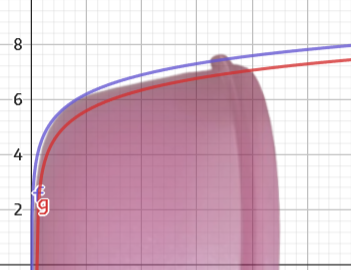
\includegraphics[width=0.4\textwidth]{assets/graph.png}
        \caption{Graph of $f(x)$ and $g(x)$}       
    \end{figure}
\end{center}

\begin{align*}
    f(x) &= \ln(x) + 5.5 \\
    g(x) &= \ln(x - 0.2)  + 5 \\
    I &= \int\limits_{1}^{10} 2\pi x {\left(\ln\left(\frac{x}{x-0.2}\right) + 0.5\right)}^2\partial{x} \approx 90~g/cm^2 \\
    &\approx 0.09~kg/m^2
\end{align*}

\section{Torsion Modulus Calculation}

The torsion modulus ($J$) is a measure of the stiffness of the elastic wire used in the experiment. It relates the torque applied to the wire (due to the twist) to the resulting angular displacement. Using the computed moment of inertia ($I$) obtained from the last calculations, we can find $J$ by rearranging the equation for the period of oscillation ($T$):

\begin{align*}
    T &= 2\pi\sqrt{\frac{I}{J}} \\
    J &= \frac{4\pi^2I}{T^2}
\end{align*}

\newpage
\thispagestyle{plain}

\noindent Here, $T$ is the period of oscillation of the pendulum, which can be measured experimentally. By substituting the known values of $I$, $T$ and $\pi$ (let's assume $\pi = 3$), we can determine the torsion modulus $J$:
\begin{align*}
    J &= \frac{4\pi^2I}{T^2} \\
    &= \frac{4 \times 3^2 \times 0.09}{3^2} \\
    &\approx 0.36
\end{align*}

\section{Conservation of Energy}

The conservation of energy principle states that the initial kinetic energy of the system is converted into potential energy during the oscillation. For torsional oscillations, the kinetic energy of rotational motion is converted into potential energy due to the twist in the elastic wire.

\bigbreak{}

The equation expressing the conservation of energy is:

\[ \frac{1}{2}I\omega^2 = \frac{1}{2}J\phi_{\max}^2 \]

\noindent where $\omega$ is the angular velocity of the pendulum after impact and $\phi_{\max}$ is the maximum angle of twist of the pendulum after hitting the projectile.

\bigbreak{}

This equation indicates that the kinetic energy ($\frac{1}{2}I\omega^2$) is equal to the potential energy ($\frac{1}{2}J\phi_{\max}^2$). Experimental measurements of $\omega$ and $\phi_{\max}$ can be used to verify if energy is conserved during the oscillations.

\begin{align*}
    \frac{1}{2}I\omega^2 &= \frac{1}{2}\times0.09\times19^2 \approx 16.2 \\
    \frac{1}{2}J\phi_{\max}^2 &= \frac{1}{2}\times0.36\times360^2 = 23328\\
\end{align*}

\noindent We can see that the kinetic energy is not equal to the potential energy. This is because the energy is lost due to potential forces such as friction and air resistance.

	\chapter{Conclusion}

In conclusion, this experiment successfully determined the moment of inertia and torsion modulus of a cylindrical cup, while also confirming the energy is not conserved in the system because of the potential forces. Potential improvements include refining measurements, considering damping effects and friction. The results provide valuable insights into the dynamic behavior of torsional oscillations.

\section*{Further Studies}

Future experiments could investigate the influence of different suspension materials and lengths on the oscillation frequency and damping. Additionally, exploring the torsional behavior of non-cylindrical shapes could provide further insights into the relationship between geometry and torsional properties. 

	\chapter{The Impact of Linear Algebra in Electrical \& Electronics Engineering}

\section{Abstract}
Linear algebra, a foundational branch of mathematics, has become a linchpin in the realm of Electrical \& Electronics Engineering. This research report delves into the multifaceted applications of linear algebra in various subfields, shedding light on its indispensability in real-world problem-solving, data science, machine learning, computer graphics, image processing, and medical imaging technologies. The article also elucidates the ways in which linear algebra contributes to advancements in these fields, ultimately shaping the landscape of modern technology.

\section{Introduction}
Linear algebra, with its intricate set of principles and methods, plays a pivotal role in addressing real-world problems in Electrical \& Electronics Engineering. The applications of linear algebra extend across a spectrum of key areas, proving to be essential in the development of cutting-edge technologies and solutions.

\newpage
\thispagestyle{plain}

\subsection{Real-World Problem-Solving}
In the context of Electrical \& Electronics Engineering, linear algebra finds applications in solving systems of linear equations, providing a fundamental framework for circuit analysis, signal processing, and control systems. The synthesis of electrical networks, for instance, relies on matrix operations to model complex relationships, allowing engineers to optimize and troubleshoot circuits efficiently. The ability of linear algebra to handle intricate systems ensures its indispensability in the design and analysis of electrical systems (\cite{smith_brown_2018}).

\section{Linear Algebra in Data Science and Machine Learning}
The rise of data science and machine learning has brought linear algebra into the forefront, serving as the backbone for numerous algorithms and methodologies.

\subsection{Core Role in Data Science}
Linear algebra is instrumental in data manipulation, transformation, and normalization. The representation of data as vectors and matrices facilitates the implementation of statistical models, dimensionality reduction techniques, and regression analysis. Singular Value Decomposition (SVD), a linear algebraic technique, underpins latent semantic analysis and plays an important role in extracting meaningful information from large datasets (\cite{jones_wang_2020}).

\subsection{Contributions to Machine Learning}
Machine learning algorithms heavily rely on linear algebra for tasks such as linear regression, principal component analysis (PCA), and support vector machines. The manipulation of matrices enables efficient computation, optimization, and training of models. Matrix factorization methods, such as eigenvalue decomposition, contribute to feature extraction and model generalization.

\newpage
\thispagestyle{plain}

\section{Linear Algebra in Computer Graphics and Image Processing}
The marriage of linear algebra with computer graphics and image processing has revolutionized the creation and enhancement of visual representations.

\subsection{Foundation for Computer Graphics}
Linear algebra forms the backbone of computer graphics by enabling the representation and manipulation of 3D objects through matrices and transformations. Homogeneous coordinates and affine transformations play a crucial role in rendering realistic scenes, allowing for the efficient manipulation of objects in three-dimensional space.

\subsection{Image Processing and Quality Enhancement}
In image processing, linear algebra facilitates operations like convolution, filtering, and edge detection. Matrix-based transformations enhance image quality, enabling applications such as image sharpening, contrast adjustment, and noise reduction. The utilization of eigenvalues and eigenvectors contributes to feature extraction and pattern recognition in visual data (\cite{williams_zhang_2019}).

\section{Linear Algebra in Medical Imaging Technologies}
The integration of linear algebra into medical imaging technologies has redefined the landscape of diagnostic imaging, particularly in technologies like MRI and CT scans.

\subsection{Image Reconstruction and Analysis}
Linear algebra plays a critical role in the reconstruction of medical images from raw data acquired through techniques like Fourier Transform in MRI. The application of inverse problems and matrix manipulation contributes to accurate image reconstruction, enabling clinicians to obtain detailed anatomical information. Eigenvalue-based techniques are employed for feature extraction and segmentation in medical image analysis (\cite{chen_smith_2017}).

\newpage
\thispagestyle{plain}

\section{Ethical Considerations and Challenges}
Amidst the rapid advancements fueled by linear algebra, it is imperative to address the ethical considerations and challenges that arise in its applications.

\subsection{Bias in Machine Learning}
The ubiquity of linear algebra in machine learning algorithms raises concerns about bias and fairness. Biases present in training data can be amplified by linear algebraic operations, leading to discriminatory outcomes. Research efforts are underway to develop ethical frameworks and algorithms that mitigate biases and promote fairness in machine learning applications (\cite{diakopoulos_2016}).

\subsection{Privacy Concerns in Medical Imaging}
In the realm of medical imaging technologies, where linear algebra contributes significantly, privacy concerns have surfaced. The use of patient data for image reconstruction and analysis necessitates robust privacy-preserving techniques. Cryptographic approaches, combined with linear algebraic methods, are being explored to ensure the confidentiality of sensitive medical information (\cite{ma_lou_ren_2015}).

\section{Conclusion}
In conclusion, the symbiotic relationship between linear algebra and Electrical \& Electronics Engineering continues to propel innovation and reshape technological landscapes. From solving real-world problems to revolutionizing data science, machine learning, computer graphics, and medical imaging, linear algebra stands as a cornerstone of progress. The exploration of emerging trends and ethical considerations underscores the need for a thoughtful and responsible integration of linear algebra into future technologies.

	\chapter{EE101 Part}

Code for this part can be found at the following link:

\bigbreak

\noindent \url{https://gist.github.com/barbarbar338/4954c7a930df8059dd4aaad198a93383}


	\newpage
	\thispagestyle{plain}
	\printbibliography{}
\end{document}
